Two Python array packages existed before NumPy.
The Numeric package began in the mid-90s and provided an array object in
Python, written in C, and linking to standard fast implementations of linear
algebra.
Around 2000, the Space Telescope Science Institute (STScI) software group wrote
a reimplementation of much of Numeric, called NumArray, to support their work
on large memory-mapped arrays and arrays of mixed data type
records \cite{STScI-slither}.
This briefly caused the two communities to diverge, until
2005, when NumPy emerged as a ``best of both worlds'' unification of Numeric
and NumArray \cite{oliphant2006guide}.

Today, NumPy underpins almost every Python library that does scientific or
numerical computation including SciPy \cite{virtanen2019scipy},
Matplotlib \cite{hunter2007matplotlib}, pandas \cite{mckinney-proc-scipy-2010},
scikit-learn \cite{pedregosa2011scikit}, and
scikit-image \cite{vanderwalt2014scikit}.
It is a community developed, open source library, which provides a
multidimensional Python array object along with array-aware functions
that operate on it.
Because of its inherent simplicity, the NumPy array is
the {\it de facto} exchange format for array data in Python.
The library has such widespread adoption that not only the array object but also its
{\it Application Programming Interface} (API) has become ubiquitous as
a language for array programming.

\section*{NumPy arrays}

\begin{figure*}
  \centering
  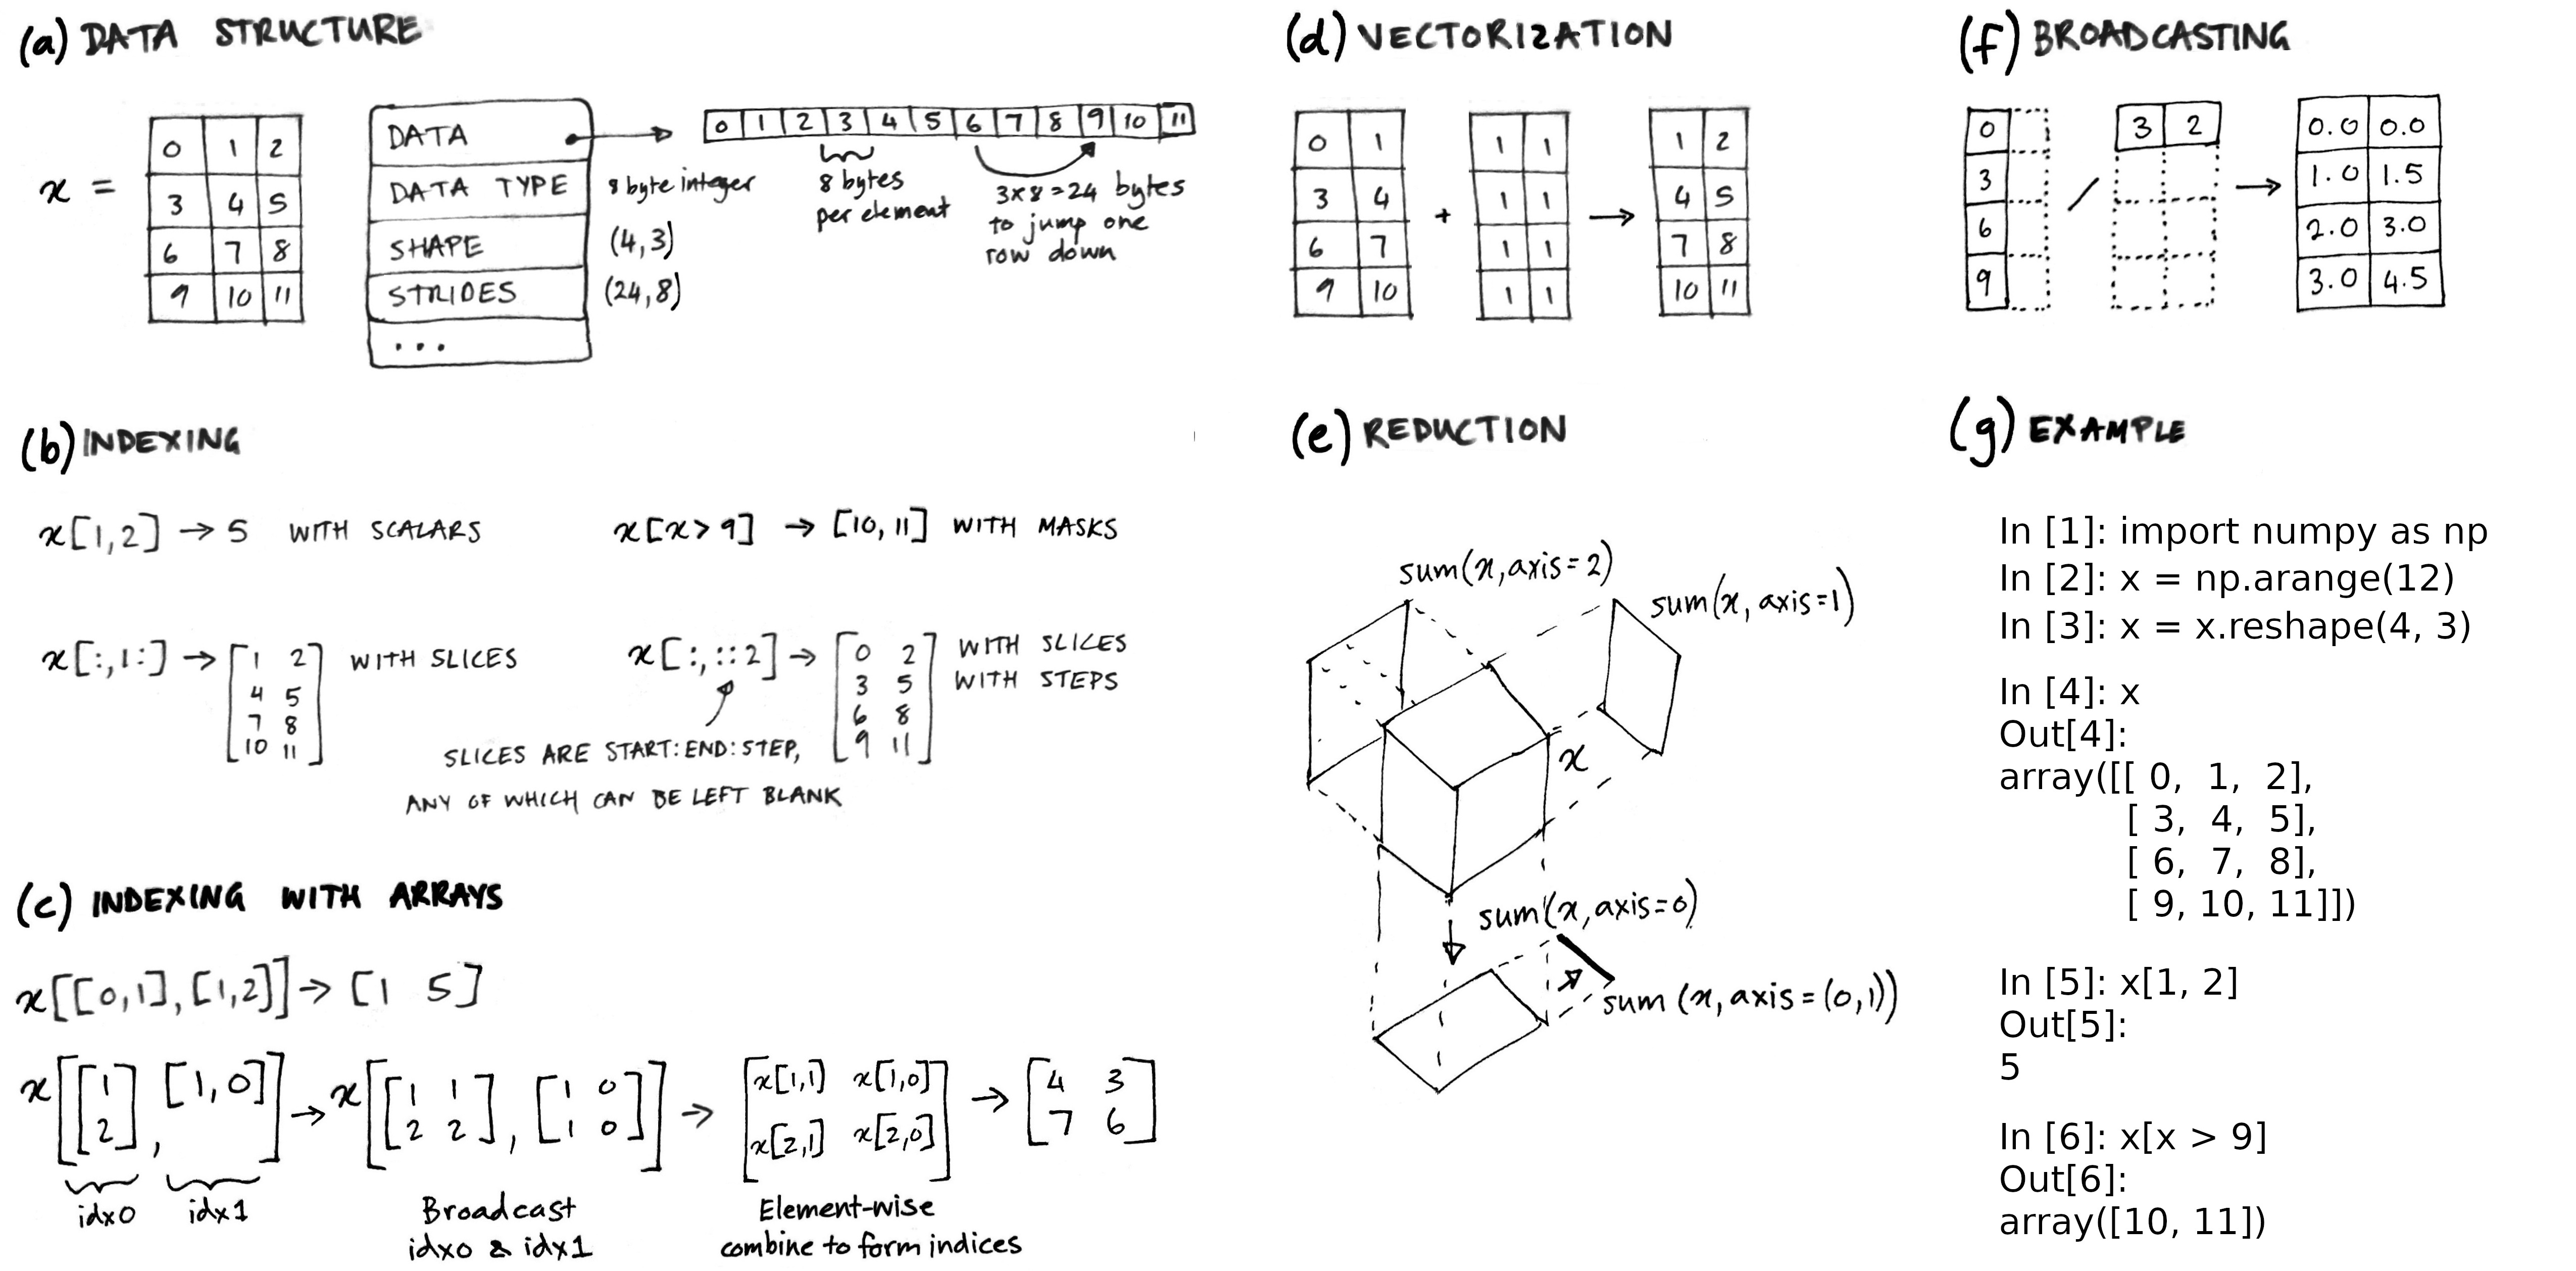
\includegraphics[width=\textwidth]{static/sketches/array-concepts}   
  \caption{\textbf{Fundamental Array Concepts.}
    \textbf{a,} The NumPy array data structure and its associated metadata fields.
    \textbf{b,} Indexing an array with various types of arguments.
    \textbf{c,} Indexing with arrays, which broadcast the indexing arguments before performing the lookup.
    \textbf{d,} Broadcasting in scalar addition, and in the division of two-dimensional arrays.
    \textbf{e,} Reduction operations act along one or more axes. In this
    example, a three-dimensional array is shown to be summed along various single
    axes to produce two-dimensional results, or along two axes consecutively to
    produce a one-dimensional result.
   }
  \label{fig:array-concepts}
\end{figure*}

The NumPy array is a data structure that efficiently stores and accesses
multidimensional arrays \cite{vanderwalt2011numpy}, also known as tensors, that
enables a wide variety of scientific computation.
It consists of a pointer to memory, along with metadata used to interpret the
data stored there, notably {\em data type}, {\em shape}, and {\em strides}
(Fig.~\ref{fig:array-concepts}a).

The \emph{data type} describes the nature of elements stored in an array.
An array has a single data type, and each array element occupies the same
number of bytes in memory.
Examples of data types include real and complex numbers (of lower and higher
precision), strings, timestamps, and pointers to Python objects.

The \emph{shape} of an array determines the number of elements along each axis,
and the number of axes is the array's dimensionality.
For example, a vector of numbers can be stored as a one dimensional array of
shape $N$, while color videos are four dimensional arrays of shape
$(T, M, N, 3)$.

\emph{Strides} are necessary to interpret computer memory, which stores elements
linearly, as multidimensional arrays.
It describes the number of bytes to move forward in memory to jump from row to
row, column to column, and so forth.
Consider, for example, a 2-D array of floating point numbers with shape
$(4, 3)$, where each element occupies 8 bytes in memory.
To move between consecutive columns we need to jump forward 8 bytes in memory,
and to access the next row $3 \times 8 = 24$ bytes.
The strides of that array are therefore $(24, 8)$.  NumPy is able to
store arrays in either C or Fortran memory order, iterating
first over either rows or columns.  This allows external libraries
written in those languages to directly access NumPy array data in memory.

Users interact with NumPy arrays using {\em indexing} (to access
subarrays or individual elements), {\em operators} (e.g., $+$, $-$, $\times$
for vectorized operations and $@$ for matrix multiplication), as well as {\em array-aware functions};
together, these provide an easily readable, expressive, high-level API for
array programming, while NumPy
deals with the underlying mechanics of making operations fast.

\emph{Indexing} an array returns single elements, subarrays, or elements that satisfy
a specific condition (Fig.~\ref{fig:array-concepts}b).
Arrays can even be indexed using other arrays (Fig.~\ref{fig:array-concepts}c).
Wherever possible, indexing that retrieves a subarray returns a {\em view} on
the original array, such that data is shared between the two arrays.
This provides a powerful way to operate on subsets of array data, while
limiting memory usage.

To complement the array syntax, NumPy includes functions that perform
\emph{vectorized} calculations on arrays, including arithmetic, statistics, and
trigonometry.
Vectorization---operating on whole arrays rather than their individual
elements---is essential to array programming.
This means that operations that would take many tens of lines to express in
languages such as C can often be implemented as a single, clear Python
expression.
This results in concise code and frees users to focus on the details of
their analysis, while NumPy handles looping over array elements near-optimally,
taking into consideration, for example, strides, in order to best utilize the
computer's fast cache memory.

When performing a vectorized operation (such as addition) on two arrays with
the same shape, it is clear what should happen.
Through \emph{broadcasting}, NumPy allows the dimensions to differ, while
still producing results that appeal to intuition.
A trivial example is the addition of a scalar value to an array, but it also
generalizes to more complex examples such as scaling each column of an array,
or generating a grid of coordinates.
In broadcasting, one or both arrays are virtually duplicated (that is, without
copying any data in memory), so that the shapes of the operands match
(Fig.~\ref{fig:array-concepts}d).
Broadcasting is also applied when an array is indexed using arrays of
indices (Fig.~\ref{fig:array-concepts}c).

Many of the array-aware functions, such as summation, support \emph{reductions}: aggregating
results across one or more dimensions of the array.
For example, summing a $n$-dimensional array over $d$ axes results in a
$(n-d)$-dimensional array (Fig.~\ref{fig:array-concepts}e).

Other array-aware functions include creating, reshaping, concatenating, and padding
arrays; searching, sorting and counting data; and reading and writing files.
NumPy provides extensive support for generating pseudorandom numbers and
includes an assortment of probability distributions.
It also performs accelerated linear algebra, utilizing one of several backends
such as OpenBLAS \cite{wang2013augem,xianyi2012model} and Intel MKL optimized for the CPUs at hand.


\section*{Scientific Python ecosystem}

SciPy and Matplotlib are tightly coupled with NumPy---in terms of
history, development, and use.
% to expand the suite of standard algorithms and
% provide basic plotting capabilities.
SciPy provides fundamental algorithms for scientific computing
including mathematical, scientific, and engineering routines.
Matplotlib generates publication-ready figures and visualizations.
The combination of NumPy, SciPy, and Matplotlib together with
an advanced interactive environment like IPython \cite{perez2007ipython}
or Jupyter \cite{Kluyver:2016aa}
provides a complete foundation for array-based scientific computing.
The scientific Python ecosystem (Fig.~\ref{fig:ecosystem}) builds on top of
this foundation to provide several, widely used \emph{technique-specific}
libraries\cite{pedregosa2011scikit,vanderwalt2014scikit,SciPyProceedings_11},
that in turn underlay numerous \emph{domain-specific} projects
\cite{astropy:2013,astropy:2018,cock2009biopython,millman2007analysis,sunpy2015,2018EGUGA..2012146H}.
NumPy, as the focal point for the ecosystem of array-aware libraries,
sets documentation standards, and provides array testing infrastructure
and build support for integrating with Fortran code and using specialized
compilers and computing platforms.

The interactive environment created by this array programming
foundation---along with the surrounding ecosystem of tools---inside of
IPython or Jupyter, is ideally suited to exploratory data analysis.
Users fluidly inspect, manipulate, and visualize their data, and
rapidly iterate to refine programming statements. These statements are
then stitched together into imperative or functional programs, or
narrative computational notebooks.  This rich and productive
environment has made the scientific Python ecosystem hugely popular
for scientific research.

Despite its tight integration, the ecosystem was conceived to have
clear functional separation, with well defined interfaces.  This makes
possible the design of large, complex scientific libraries, that
add specialized functionality for solving specific problems.

%As a result, important scientific software
%packages build on the ecosystem, and further expand it for specific
%research projects.

\begin{figure}
  \centering
  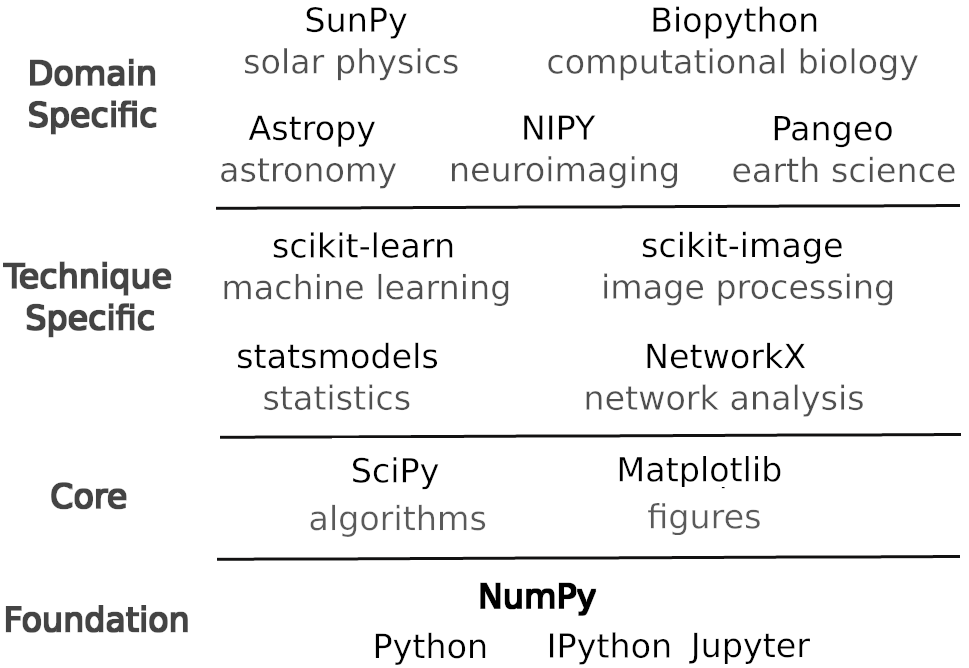
\includegraphics[width=.45\textwidth]{static/ecosystem}
  \caption{\textbf{Scientific Python Ecosystem.}
   This figure highlights some of the essential tools and libraries in the vast
   scientific Python ecosystem.  Most of the ecosystem builds on NumPy to
   provide a rich and powerful collection of array-aware functionality.
  }
  \label{fig:ecosystem}
\end{figure}

For example, the \code{eht-imaging} library developed by the Event Horizon Telescope 
collaboration relies on many components of the scientific Python ecosystem.
NumPy arrays are used to store and manipulate numerical data at every step
in the processing chain: from raw data through calibration and image 
reconstruction.
SciPy is used to provide tools used in general image processing such as 
filtering and image alignment, while scikit-image---a popular image processing
library that extends SciPy---provides higher-level functionality such as
edge filters and Hough transforms.
Other components of SciPy are used throughout the library, such as the
\code{scipy.optimize} module for handling general optimization tasks.
NetworkX \cite{SciPyProceedings_11}---a popular package for complex
network analysis---is used for analysis of consistency among image
comparisons.
The community-developed astronomy library, Astropy \cite{astropy:2013, astropy:2018},
is used throughout \code{eht-imaging}, primarily to handle standard
astronomical file formats and time/coordinate transformations.
Matplotlib is used for visualizing data throughout the analysis pipeline,
including the generation of the final image of the black hole.

Similar examples can be found in physics, earth science, biology,
and more.
% FIXME: this should be expanded 
Over the last few years there has been a massive increase in the use
of scientific Python due in part to the rapid growth of data science,
machine learning, and artificial intelligence.  
As a result, NumPy and its API has become ubiquitous.


\section*{Proliferation of arrays}

NumPy provides in-memory, multidimensional, homogeneously typed
(i.e., single pointer and strided) arrays on CPUs.
It supports many types of CPUs (e.g., POWER and ARM) with similar
performance as native C code.
% a brief word about accelerators perhaps?
% end with how this fits the bill for a huge number of users

While NumPy suits most user's needs, it cannot support every specialized need
of the community; due to its in-memory data model, it is limited in its ability
to work with very large datasets, datasets split across multiple systems, and
computations that require graphics processing units (GPUs), tensor processing
units (TPUs) or other specialized hardware for performance reasons.

% maybe mention that there are typically utilities
% to convert to and from numpy arrays
% and why (presumably to get access to ecosystem)
The community's efforts to fill the resultant gaps led to a
proliferation of array implementations. Each deep learning framework created
its own arrays; PyTorch \cite{NEURIPS2019_9015},
Tensorflow \cite{abadi2016tensorflow}, Apache MXNet \cite{chen2015mxnet},
and JAX \cite{jax2018github} arrays all have the
capability to run on CPUs and GPUs, in a distributed fashion, and in a delayed
execution mode to allow for performance optimizations.  SciPy and Sparse both
provide sparse arrays---which typically contain few non-zero values and store
only those in memory for efficiency.
In addition there are projects that build on top of NumPy arrays as a data
container and \textit{extend} its capabilities.  Distributed arrays are
made possible that way by Dask, and labeled arrays---referring to dimensions of
an array by name rather than by index for clarity, compare \code{x[:,~1]} vs.
\code{x.loc[:,~'time']}---by Xarray \cite{hoyer2017xarray}.

Importantly, some projects chose to follow the NumPy API exactly---with Dask,
CuPy, Sparse and JAX the most prominent examples---while others have
NumPy-inspired semantics but chose to deviate in places.
% when they deviate, they sometimes fix it, e.g.,
% https://github.com/pytorch/pytorch/pull/1983
% https://github.com/pytorch/pytorch/issues/2228
% many have for numpy users
% https://github.com/torch/torch7/wiki/Torch-for-Numpy-users

% computation graphs---which postpone and combine calculations
% before executing them efficiently,

Ideally, operating on these arrays using NumPy functions or semantics would
simply work, so that end users could write code once, and would then benefit
from switching between NumPy arrays, GPU arrays, distributed arrays, and so
forth, as appropriate.
To support array operations between external array objects, NumPy
acts as a central coordination mechanism with a well-specified API.
The widespread adoption of the NumPy API is valuable: it lowers the
barrier to entry for newcomers and provides the wider community with a
stable array programming interface. This, in turn, prevents disruptive
schisms like the divergence of Numeric and NumArray, by facilitating
the development of specialized solutions and new tools that operate in
concert.

\begin{figure}
  \centering
  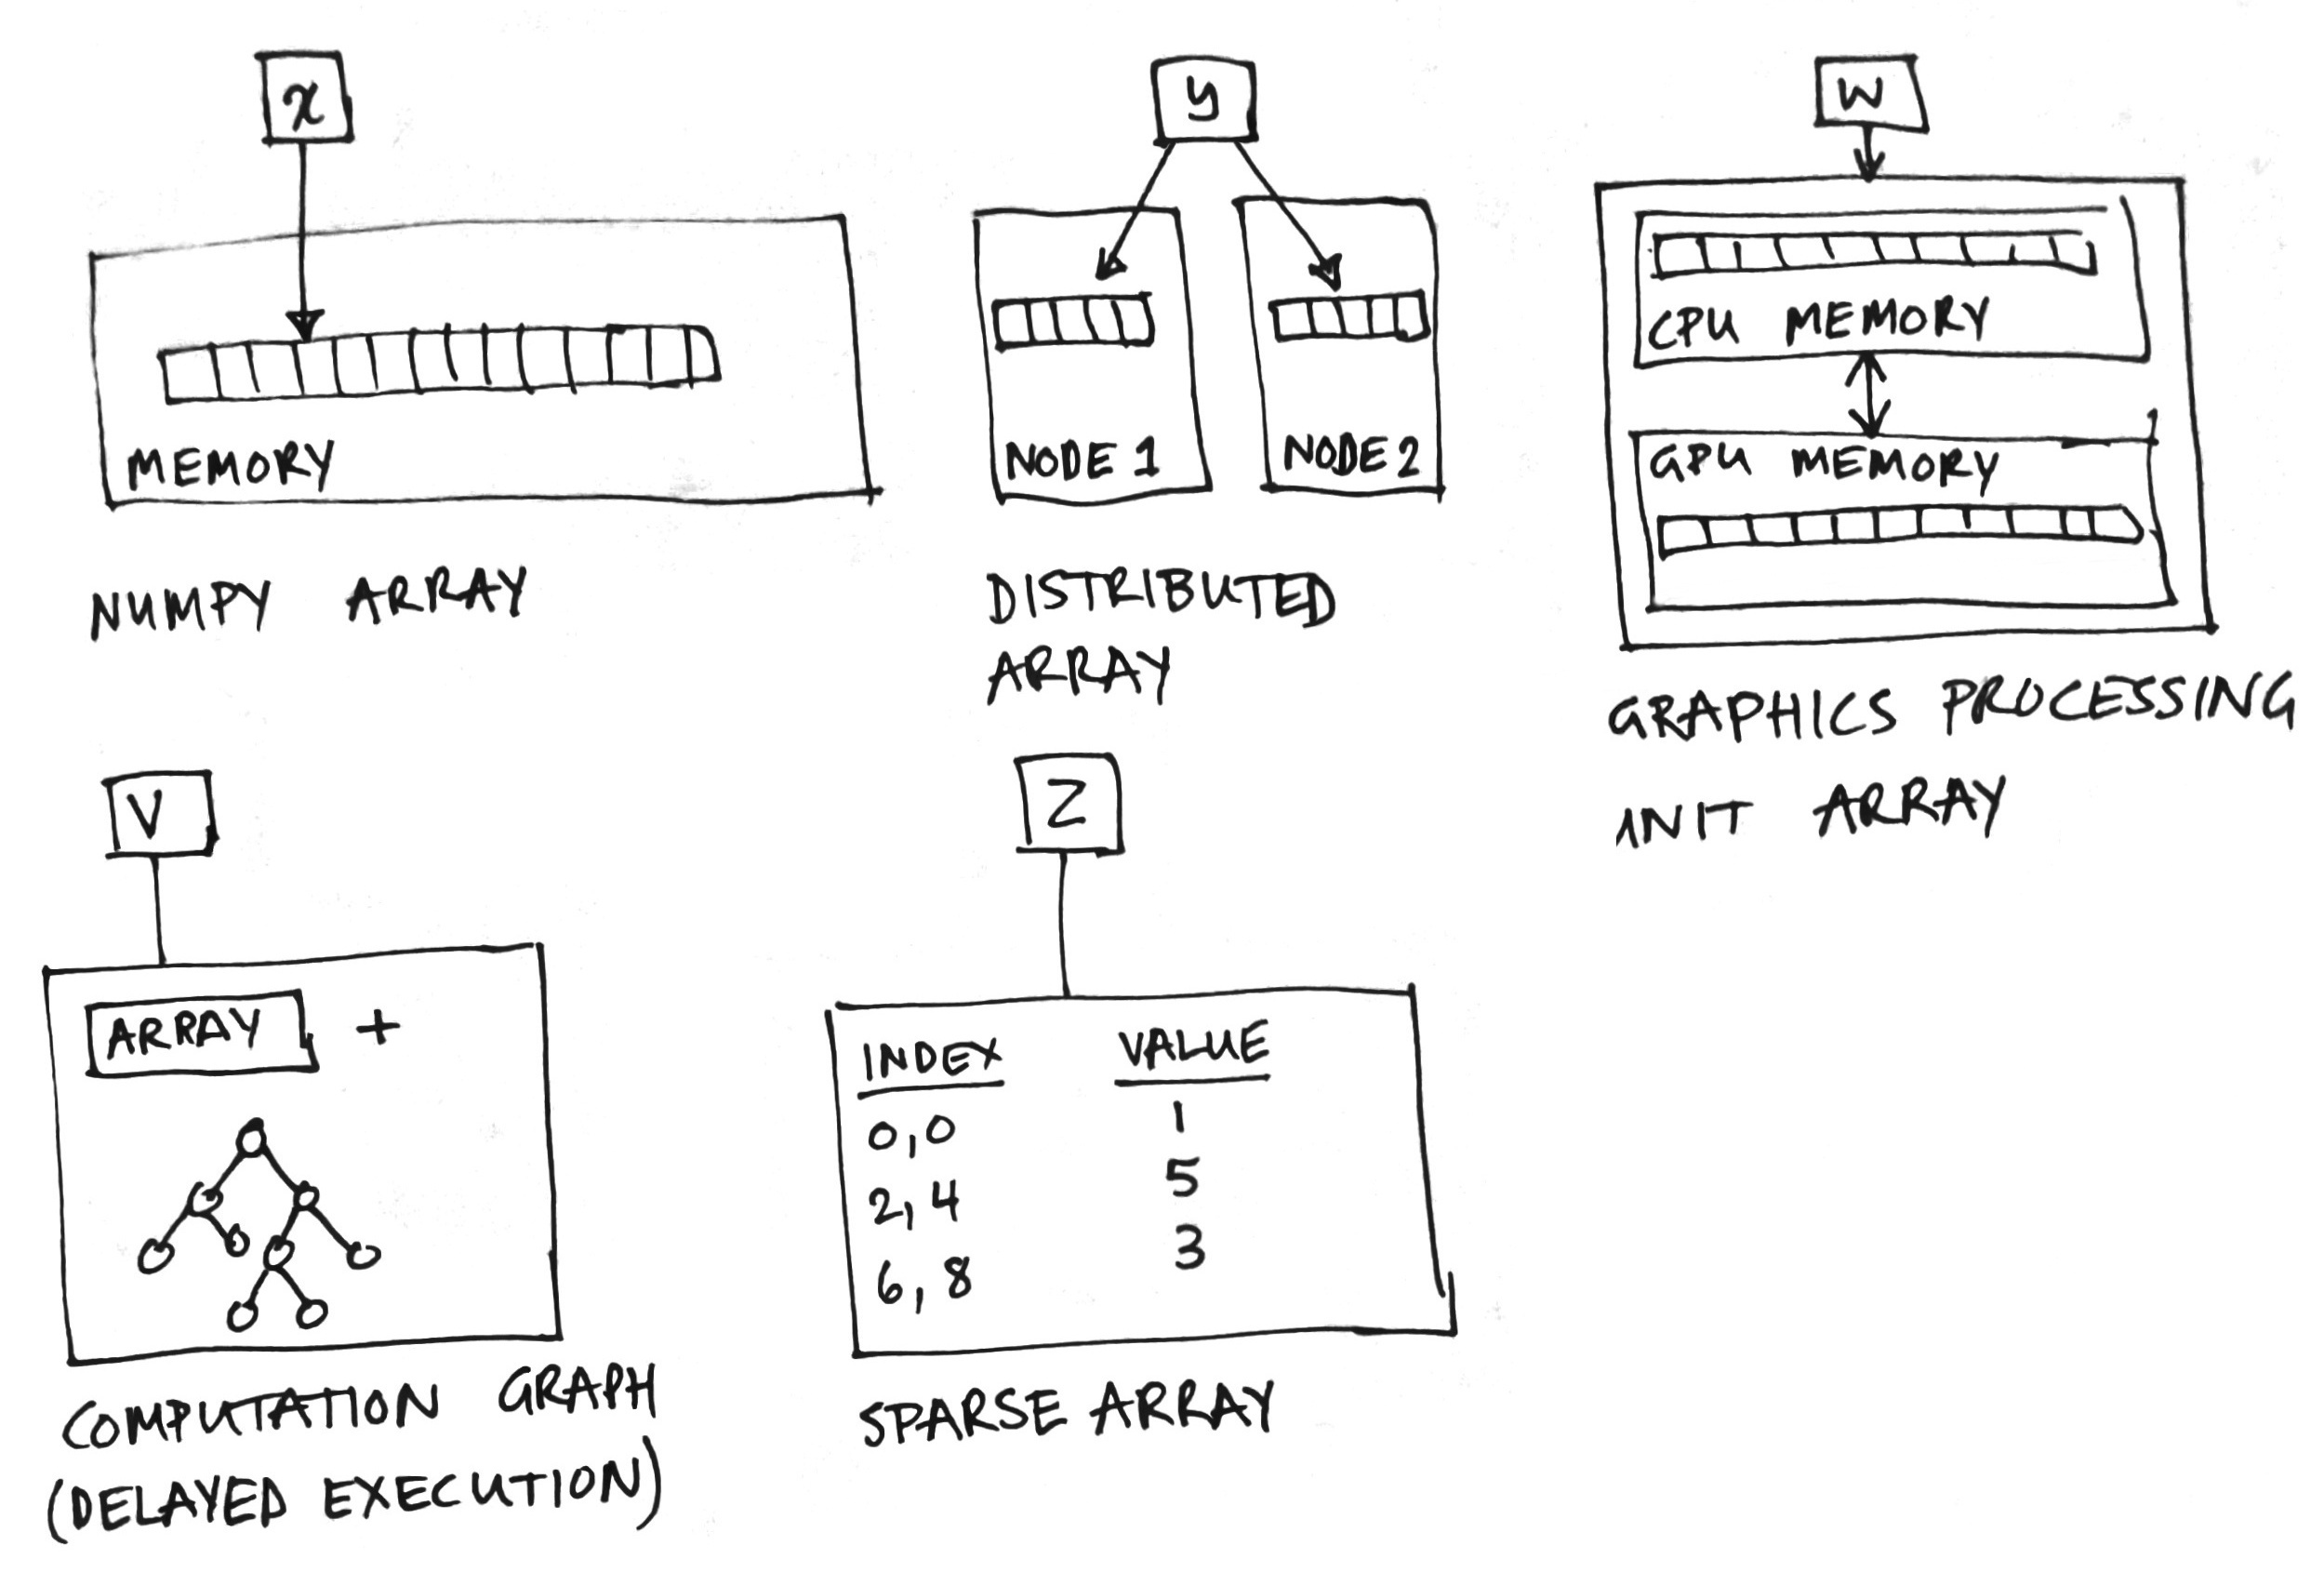
\includegraphics[width=.45\textwidth]{static/sketches/duck-arrays}
  \caption{\textbf{Interoperability.} \fixme{This figure needs work.}}\label{fig:duck-arrays}
\end{figure}

% should we hint at some of the community interaction part
% they have helped us develop the neps and e.g.,
% https://github.com/pytorch/pytorch/issues/22402
To facilitate \emph{interoperability}, NumPy provides
``protocols'' (or contracts of operation), that allow for these arrays to be
passed to NumPy functions (Fig.~\ref{fig:duck-arrays}).
NumPy, in turn, dispatches operations to the originating library, as required.
% FIXME: expand to 3 or more sentences discussing current efforts and
% issues with those, how did adoption go, what is being done next
%\url{https://numpy.org/neps/nep-0037-array-module.html}
Versions of these protocols have been successfully deployed.
% Ralf: Could you provide some proof of effectiveness, e.g., "This has made it
% possible to create distributed GPU arrays, enabling .... [find a reference to
% work by Peter Entschev]".
% Best reference: https://ep2019.europython.eu/talks/fX8dJsD-distributed-multi-gpu-computing-with-dask-cupy-and-rapids/
% Below an attempt to start on this:
Thanks to these developments users of Dask and NumPy arrays are now capable
of scaling their computation to the GPU using Dask's CuPy integration with
only minimal code changes.
% spelled out on this page: https://docs.dask.org/en/latest/gpu.html
% The video cited embedded there could be a citation:i
% https://on-demand-gtc.gputechconf.com/gtcnew/sessionview.php?sessionName=s9198-dask+and+v100s+for+fast%2c+distributed+batch+scoring+of+computer+vision+workloads
However, general adoption has not yet been achieved mainly for compatibility
concerns.
% explain a bit what "compatibility concerns" means ...
Thus, we are actively addressing these concerns by revising and extending
these protocols with the aim of wide interoperability that spans the whole
scientific Python ecosystem up to and including domain libraries.

% https://numpy.org/neps/nep-0016-abstract-array.html
% https://numpy.org/neps/nep-0018-array-function-protocol.html
% https://numpy.org/neps/nep-0022-ndarray-duck-typing-overview.html
% https://numpy.org/neps/nep-0030-duck-array-protocol.html
% https://github.com/numpy/numpy/blob/a111b551ae940d7d5f8523fef1cf3589c6ba00a0/doc/neps/nep-0033-extensible-dtypes.rst
% https://numpy.org/neps/nep-0037-array-module.html

\section*{Discussion}

NumPy was initially developed by students, faculty, and researchers to
provide an advanced, open source array programming library for Python,
which was free to use and unencumbered by license servers, dongles, and the like.
There was a sense of building something
impactful together, for the benefit of many others.  Participating in
such an endeavor, within a welcoming community of like-minded
individuals, held a powerful attraction for many early contributors.

These user-developers frequently had to write code from scratch to solve
their or their colleagues' problems---often in low-level languages
that preceded Python, like Fortran \cite{dongarra2008netlib} and C.
To them, the advantages of an interactive, high-level array library
were evident. The design of this new tool was informed by their
experiences with powerful interactive programming languages for
scientific computing such as APL \cite{iverson1962programming} and
Yorick \cite{munro1995using}, as well as commercial languages and
environments like IDL and Matlab.

NumPy has subsequently seen prolific adoption, with millions of users,
first from research and later also industry.
It spurred the development of the larger scientific Python ecosystem and
heralded the current era of wide-spread use of Python for scientific computing.
The reasons for its popularity are varied and complex, but include the fact that
NumPy (a) is built on top of Python,
(b) has a strong culture of collaboration and good software development practices, and
(c) provides a cutting-edge array programming environment for scientific data analysis.

\emph{Python} is an open source, general-purpose, interpreted programming language
well-suited to standard programming tasks such as cleaning data,
interacting with web resources, and parsing text.
Adding fast array operations and linear algebra allows scientist to do all
their work within a single language---and one that has the advantage of
being famously easy to learn and teach.
In fact, Python's adoption as a primary learning language in universities
(e.g., many lower division UC Berkeley courses use Python including
Foundations of Data Science,
The Beauty and Joy of Computing,
Introduction to Computational Thinking with Data,
and The Structure and Interpretation of Computer Programs) has
further popularized NumPy as a tool of choice for modern data science.

Even though NumPy is not part of Python's standard library,
we benefit from a good relationship with the Python developers.
Over the years, the Python language has added new features and
special syntax so that NumPy would have more succinct and 
easy to read array notation.
Since we are not part of the standard library, we are able to
dictate our own release policies and development patterns.
%\fixme{we've gotten a number of features: slicing syntax, implicit tuples,
%complex numbers, buffer protocol, matrix multiplication operator}
%\fixme{but we benefit from separate governance}

NumPy is a community of practice with a strong \emph{culture} of
employing software engineering practice to improve collaboration and
reduce error \cite{millman2014developing}.  This culture is not only
adopted by leaders in the project, but also enthusiastically taught to
newcomers. The NumPy team was early in adopting distributed revision
control and code review to improve collaboration on code, and
continuous testing that runs a large battery of automated tests for
every proposed change to NumPy.  The project has comprehensive,
high-quality documentation, integrated with the source
code \cite{vanderwalt2008scipy,harrington2008scipy,harrington2009scipy}.

% https://ras.ac.uk/sites/default/files/2020-01/Group%20Award%20-%20Astropy.pdf
% https://ras.ac.uk/news-and-press/news/leading-astronomers-and-geophysicists-honoured-ras-bicentenary-year-0

This culture of using best practices for producing reliable scientific software
has been adopted by the ecosystem of libraries that build on NumPy.
For example, in a recent award given by the Royal Astronomical Society to
Astropy, they state:
\begin{quotation}
\noindent\emph{The Astropy Project has provided hundreds of junior scientists
with experience in professional-standard software development practices
including use of version control, unit testing, code review and issue tracking
procedures. This is a vital skill set for modern researchers that is often
missing from formal university education in physics or astronomy.}
\end{quotation}
Community members explicitly work to address this lack of formal education
through formal courses and workshops
\cite{wilson-software-carpentry,hannay-scientific-software-survey,millman2018teaching}.

NumPy combines the expressive power of \emph{array programming}, 
the performance of C, and
the readability, usability, and versatility of Python in a mature,
well-tested, well-documented, and community developed library.
It builds on decades of work refining the array programming
syntax from APL through Yorick and others.
It also made it easy for other libraries to develop fast and
memory-efficient compiled code, usually in C or Fortran, that could manipulate
these arrays and pass them back to Python.
Popular array-aware libraries increased the user community and that
in turn led to more libraries adding new functionality
to the scientific Python ecosystem.

Over time the role of the NumPy has evolved.
It began as an attempt to add an array object to Python
and became the foundation of a rich ecosystem of tools.
Now a large amount of scientific work depends on NumPy
being correct, fast, and stable.
Yet, it is no longer just the foundational array library underlying the
scientific Python ecosystem; it is also a standard API for tensor
computation and a central coordinating mechanism between array types and
technologies.
